%You can leave alone everything before Line 79.
\documentclass{article}
\usepackage{url,amsfonts, amsmath, amssymb, amsthm,color, enumerate, verbatim}
% Page layout
\setlength{\textheight}{8.75in}
\setlength{\columnsep}{2.0pc}
\setlength{\textwidth}{6.5in}
\setlength{\topmargin}{0in}
\setlength{\headheight}{0.0in}
\setlength{\headsep}{0.0in}
\setlength{\oddsidemargin}{0in}
\setlength{\evensidemargin}{0in}
\setlength{\parindent}{1pc}
\newcommand{\shortbar}{\begin{center}\rule{5ex}{0.1pt}\end{center}}
%\renewcommand{\baselinestretch}{1.1}
% Macros for course info
\newcommand{\courseNumber}{ME 552}
\newcommand{\courseTitle}{Mechatronics}
\newcommand{\semester}{Fall 2012}
\newcommand{\xxx}[1]{\textcolor{red}{#1}}
% Theorem-like structures are numbered within SECTION units
\theoremstyle{plain}
\newtheorem{theorem}{Theorem}[section]
\newtheorem{lemma}[theorem]{Lemma}
\newtheorem{corollary}[theorem]{Corollary}
\newtheorem{proposition}[theorem]{Proposition}
\newtheorem{statement}[theorem]{Statement}
\newtheorem{conjecture}[theorem]{Conjecture}
\newtheorem{fact}{Fact}
%definition style
\theoremstyle{definition}
\newtheorem{definition}[theorem]{Definition}
\newtheorem{example}{Example}
\newtheorem{problem}[theorem]{Problem}
\newtheorem{exercise}{Exercise}
\newtheorem{algorithm}{Algorithm}
%remark style
\theoremstyle{remark}
\newtheorem{remark}[theorem]{Remark}
\newtheorem{reduction}[theorem]{Reduction}
%\newtheorem{question}[theorem]{Question}
\newtheorem{question}{Question}
%\newtheorem{claim}[theorem]{Claim}
%
% Proof-making commands and environments
\newcommand{\beginproof}{\medskip\noindent{\bf Proof.~}}
\newcommand{\beginproofof}[1]{\medskip\noindent{\bf Proof of #1.~}}
\newcommand{\finishproof}{\hspace{0.2ex}\rule{1ex}{1ex}}
\def\therefore{\boldsymbol{\text{ }
\leavevmode
\lower0.4ex\hbox{$\cdot$}
\kern-.5em\raise0.7ex\hbox{$\cdot$}
\kern-0.55em\lower0.4ex\hbox{$\cdot$}
\thinspace\text{ }}}

\newenvironment{solution}[1]{\medskip\noindent{\bf Problem #1.~}}{\shortbar}

%====header======
\newcommand{\solutions}[4]{
%\renewcommand{\thetheorem}{{#2}.\arabic{theorem}}
\vspace{-2ex}
\begin{center}
{\small  \courseNumber, \courseTitle
\hfill {\Large \bf {#1} }\\
\semester, University of Michigan, Ann Arbor \hfill
{\em Date: #3}}\\
\vspace{-1ex}
\hrulefill\\
\vspace{4ex}
{\LARGE Lab Assignment #2}\\
\vspace{2ex}
\end{center}
\begin{trivlist}
\item \textsc{Team members:\\} {#4}
\end{trivlist}
\noindent
\shortbar
\vspace{3ex}
}
% math macros
\newcommand{\defeq}{\stackrel{\textrm{def}}{=}}
\newcommand{\Prob}{\textrm{Prob}}
\newcommand{\Lagr}{\mathcal{L}}
\newcommand{\Sens}{\mathcal{S}}
%==
\usepackage{graphicx}
\usepackage{xfrac}
\usepackage{amsmath}
\providecommand{\e}[1]{\ensuremath{\times 10^{#1}}}
\begin{document}
%%%%%%%%%%%%%%%%%%%%%%%%%%%%%%%%%%%%%%%%%%%%%%%%%
%\solutions{Your name}{Problem Set Number}{Date of preparation}{Collaborators}{Prover}{Verifiers}
\solutions{}{6: Inertial Sensors}{\today}{Shiva Ghose, @gshiva\\ John Peterson, @jrpeters\\ Peter Turpel, @pturpel\\ Chan-Rong Lin, @pmelin}
%%%%%%%%%%%%%%%%%%%%%%%%%%%%%%%%%%%%%%%%%%%%%%%%%
%\renewcommand{\theproblem}{\arabic{problem}} 
%%%%%%%%%%%%%%%%%%%%%%%%%%%%%%%%%%%%%%%%%%%%%%%%%
%
% Begin the solution for each problem by
% \begin{solution}{Problem Number} and ends it with \end{solution}
%
% the solution for Problem 
\section*{Teamwork Participation Pledge :: Team 1}

I attest that I have made a fair and equitable contribution to this lab and submitted 
assignment. \\

My signature also indicates that I have followed the University of Michigan Honor Code, 
while working on this lab and assignment.\\

I accept my responsibility to look after all of the equipment assigned to me and my team, 
and that I have read and understood the X50 Lab Rules.\\

\begin{table}[h]
\begin{center}
    \begin{tabular}{|c|c|c|}
        \hline
        \textbf{Name} & \textbf{Email}     & \textbf{ \ \ \ \ \  \ \  \ \ \ \ \  \ \ Signature  \ \ \ \ \  \ \ \ \ \ \ \  \ \ } \\ \hline
        	~& ~& ~\\
	~& ~& ~\\
	Shiva Ghose   & gshiva@umich.edu   & ~                  \\
	~& ~& ~\\
	~& ~& ~\\ \hline 
	~& ~& ~\\
	~& ~& ~\\
        John Peterson & jrpeters@umich.edu & ~                  \\ 
	~& ~& ~\\
	~& ~& ~\\ \hline 
	~& ~& ~\\
	~& ~& ~\\
        Peter Turpel   & pturpel@umich.edu & ~                  \\
	~& ~& ~\\
	~& ~& ~\\ \hline 
	~& ~& ~\\
	~& ~& ~\\
        Chan-Rong Lin   & pmelin@umich.edu & ~                  \\
	~& ~& ~\\
	~& ~& ~\\ \hline 
        \hline
    \end{tabular}
\end{center}
\end{table}

\newpage

\section{Accelerometer Wiring \& Configuration} 

\subsection{Configuration}

The accelerometer is mounted to a breadboard fixed to the the shaft clamp on the encoder such that the plane of the sensor PCB is perpendicular to the plane of axis of rotation of the encoder.  This is necessary because of the limited number of axes available on the rate gyro.  For this assignment we will be making use of the Y and Z axes of the accelerometer and the \xxx{AXIS} axis of the rate gyro.  \\

\xxx{Confirm that the wiring diagram is correct specifically whether we are using the high or low sensitivity outputs.}

\xxx{Still missing gyro details}

\xxx{We may want a picture of each axis including gyro}

\clearpage

\section{Modeling Assumptions}
% there is probably more stuff
\begin{itemize}
\item{Assume that outputs of each axis of the accelerometer and the gyro are independent of one another}
\end{itemize}

\section{Parameter Identification}

The basic behavior of an accelerometer, sensitive in the $\hat{u}$ direction is given by equation \ref{ParamID_EQ1} for quasi-static accelerations.  Where $V_{out}$ is the output voltage of the sensor,$V_{bias}$ is the output of the sensor under no acceleration, $V_{supply}$ is the supply voltage to the sensor, and $\Sens$ is a linear approximation of sensor behavior.

\begin{equation}
V_{out} = V_{bias} + \Sens \ddot{u} \quad V_{bias} \approx \frac{V_{supply}}{2}
\label{ParamID_EQ1}
\end{equation}

This response to acceleration can be also be used to measure the acceleration due to gravity along the sensitive axis of an accelerometer allowing the angle between the accelerometer and vertical to be determined.  Let $\theta$ be the measured angle from vertical to the $\hat{y}$ direction of our system.  We can consider two situations, when the sensitive axis is aligned with $\hat{y}$ axis and when it is perpendicular to it.  Let $Y$ and $Z$ denote these situations respectively which correspond to the $\hat{y}$ and $\hat{z}$ axes of our accelerometer.  Then the output voltage of each axis is given as follows:

\begin{equation}
V_{Y} = V_{Ybias} + \Sens_{Y} g \cos(\theta) \quad V_{Z} = V_{Zbias} + \Sens_{Z} g \sin(\theta)
\label{ParamID_EQ2}
\end{equation}

\begin{figure}
\begin{center}
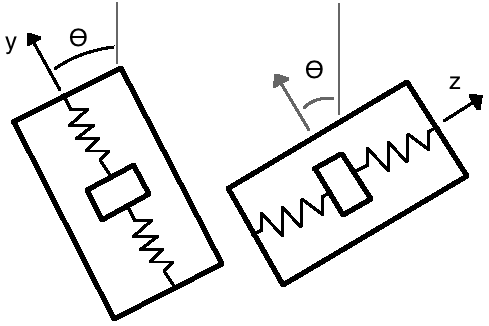
\includegraphics[width = 11cm]{Accelerometer_Cartoon.png}
\caption{Y and Z axis accelerometer}
\label{Accel_cartoon}
\end{center}
\end{figure}

\xxx{need two pictures of the cartoon proof mass}

We measured the bias voltage of each axis by fixing the accelerometer such that the axis was perpendicular to the force of gravity and recording the voltage output.  We obtained the bias voltage by averaging these voltages, and we also obtained a measure of noise along each axis by computing the variance of the obtained voltages.  We then conducted a simple experiment where the accelerometer was rotated at slow speeds throughout a complete circle while both axis voltage outputs and encoder angle measurements were recorded.  The equations in \ref{ParamID_EQ2} are linear in the sensitivity values, so we obtained each value through simple least squares regression.  These results are shown in table \ref{ParamID_T} \xxx{not the right table?} \\

\xxx{units for variance}
% values as reported by matlab SY = 0.034002931081677, SZ = 0.033903141625302, EY = 2.642681255078259\e{-5}, EZ = 2.774354019095888\e{-4}
\begin{table}
\begin{center}
    \begin{tabular}{|c|c|c|}
        \hline
        Axis                              & Y                     & Z                     \\ \hline
        $V_{bias} \, (V)$                        & 1.617433958           & 1.671451851           \\ 
        $\sigma^2 \, (V^2)$                        & 1.24553\e{-5}           & 0.001852504           \\ 
        $\Sens \, \left(\sfrac{V s^2}{m} \right)$                           & $0.03400293$     & $0.03390314$     \\ 
        Fitting Error $(V)$ & $2.642681\e{-5}$ & $2.774354\e{-4}$ \\
        \hline
    \end{tabular}
\label{ParamID_T}
\caption{Fitting error denotes average error per sample}
\end{center}
\end{table}

We see that as reported in the data sheet, the Z-axis is noisier than the Y-axis, but it is to a much greater degree than the data sheet would suggest.  We also see that this extra noise is reflected in the higher fitting errors for the Z-axis data.  


\clearpage
\section{Low Frequency Characterization}

%%%%%%%%%%%%%%%%%%%%%%%%%%%%%%%%%%%%%%%%%%%%%%%%%%%%%%%%%
\subsection{Horizontal Accelerometer}

\subsubsection{Angle Measurement}

Using a single accelerometer in the horizontal configuration is equivalent to just using the Z axis in our configuration.  Where $V_{Z}$ is given as follows: 

$$ V_{Z} = V_{Zbias} + \Sens_{Z} g \sin(\theta) $$

$\theta$ can be easily computed by the following expression:

\begin{equation}
\theta = \sin^{-1}\left( \frac{V_{Z} - V_{Zbias}}{\Sens_{Z} g}\right) 
\label{horizontalEQ}
\end{equation}

When using a single accelerometer in the horizontal configuration aliasing occurs for $|\theta| \geq \sfrac{\pi}{2}$.

\xxx{Signal Conditioning?}

\subsubsection{Sensitivity}

The relationship between sensor output voltage and angle is non-linear, but we are able to linearize about a particular operating point, for this experiment, $\theta = 0$, and obtain an estimate of the sensitivity.

$$ V_{Z} \approx V_{Zbias} + \Sens_{Z} g \sin(0) + \Sens_{Z} g \cos(0) \left(\theta - 0\right) = V_{Zbias} + \Sens_{Z} g \theta $$

For the horizontal accelerometer, we expect the sensitivity to be $\Sens_{Z} g$. 

\xxx{still need the real results here?}

\subsubsection{Noise}

An estimate for the expected noise in measurement of $\theta$ can be obtained by performing a variance projection through the partial derivative of equation \ref{horizontalEQ}.

$$ \frac{\partial \theta}{\partial V_{Z}} =  \frac{1}{\sqrt{(\Sens_{Z} g)^2 - (V_{Z} - V_{Zbias})^2}}$$

$$ \sigma^2_{\theta} = \frac{\partial \theta}{\partial V_{Z}} \sigma^2_{V_{Z}} \frac{\partial \theta}{\partial V_{Z}} $$

$$ \sigma^2_{\theta} = \frac{\sigma^2_{V_{Z}}}{(\Sens_{Z} g)^2 - (V_{Z} - V_{Zbias})^2}$$

For $\theta \approx 0$ we would expect the noise of our angle measurements to be given by:

$$ \theta \approx 0 \quad \sigma^2_{\theta} \approx \frac{\sigma^2_{V_{Z}}}{(\Sens_{Z} g)^2}$$

% we could plot \sigma^2_theta with respect to theta if we wanted to
\xxx{need to compare to real noise about this point, but our math should be exactly correct}

%%%%%%%%%%%%%%%%%%%%%%%%%%%%%%%%%%%%%%%%%%%%%%%%%%%%%%%%%
\subsection{Vertical Accelerometer}

\subsubsection{Angle Measurement}

Using a single accelerometer in the vertical configuration is equivalent to using just the Y axis in our configuration.  Where $V_{Y}$ is given as follows:

$$ V_{Y} = V_{Ybias} + \Sens_{Y} g \cos(\theta) $$

Then $\theta$ is given by the following expression:

\begin{equation}
\theta = \cos^{-1}\left( \frac{V_{Y} - V_{Ybias}}{\Sens_{Y} g}\right)
\label{verticalEQ}
\end{equation}

When using a single accelerometer in this configuration aliasing occurs for angles beyond the range $0 \leq \theta \leq \pi$.  This range is much less useful than the range for a single accelerometer in the horizontal configuration because we are unable to read negative angles immediately next to our starting condition, $\theta = 0$. 

\xxx{Signal Conditioning?}

\subsubsection{Sensitivity}

However attempting to linearize about $\theta = 0$ for the accelerometer in the vertical configuration is not nearly as successful.  Yielding a relationship that does not depend on $\theta$ at all.  This result is expected from our earlier assesment of the angle ambiguity between positive values of $\theta$ and negative values.  

$$V_{Y} \approx V_{Ybias} + \Sens_{Y} g \cos(0) - \Sens_{Y} g \sin(0) (\theta - 0) = V_{Ybias} + \Sens_{Y} g $$

\xxx{still need the real results here}

\subsubsection{Noise}

We can again use variance projection to estimate the noise in our angle measurements, taking the partial derivative of equation \ref{verticalEQ}.

$$ \frac{\partial \theta}{\partial V_{Y}} = -\frac{1}{\sqrt{(\Sens_{Y} g)^2 - (V_{Y} - V_{Ybias})^2}}$$

$$ \sigma^2_{\theta} = \frac{\partial \theta}{\partial V_{Y}} \sigma^2_{V_{Y}} \frac{\partial \theta}{\partial V_{Y}} $$

$$ \sigma^2_{\theta} = \frac{\sigma^2_{V_{Y}}}{(\Sens_{Y} g)^2 - (V_{Y} - V_{Ybias})^2}$$

As we would expect, this appears identical to the equation for noise of the horizontally mounted accelerometer.  The difference in behavior is simply the voltage around which we linearize.  Substituting the value for $V_{Y}$ about $\theta = 0$  yields absolutely terrible data compared to the horizontal case.

% is this result just a quirk of the linearization?

$$ \theta \approx 0 \quad \sigma^2_{\theta} \approx \frac{\sigma^2_{V_{Y}}}{(\Sens_{Y} g)^2 - (V_{Ybias} + \Sens_{Y} g - V_{Ybias})^2} = \infty$$



%%%%%%%%%%%%%%%%%%%%%%%%%%%%%%%%%%%%%%%%%%%%%%%%%%%%%%%%%
\subsection{Two Accelerometers}

\subsubsection{Angle Measurement}

We can overcome the aliasing issue  presented in the two configuration by using both the horizontal and vertical, the Z and Y axis, simultaneously.  

$$ \cos(\theta) = \frac{V_Y-V_{Ybias}}{\Sens_{Y} g} \quad \sin(\theta) = \frac{V_{Z} - V_{Zbias}}{\Sens_{Z} g} $$

Combining the two equations gives the following:

$$ \tan(\theta) = \frac{\sin(\theta)}{\cos(\theta)} = \left(\frac{V_{Z} - V_{Zbias}}{\Sens_{Z} g}\right) \left( \frac{\Sens_{Y} g}{V_Y-V_{Ybias}} \right) = \frac{\Sens_{Y}}{\Sens_{Z}} \left( \frac{V_{Z} - V_{Zbias}}{V_{Y} - V_{Ybias}} \right)$$

Using the atan2 function avoids the quadrant ambiguities present in the ordinary $\tan^{-1}$ function giving us an expression for $\theta$ valid for all angles.

$$\theta = \text{atan2}\big( \Sens_{Y} \left( V_{Z} - V_{Zbias}\right),  \Sens_{Z} \left( V_{Y} - V_{Ybias}\right) \big)$$

\xxx{Signal Conditioning?}

\subsubsection{Sensitivity}

\subsubsection{Noise}

$$ \theta = \tan^{-1} \left( \frac{\Sens_{Y} \left( V_{Z} - V_{Zbias}\right)}{\Sens_{Z} \left( V_{Y} - V_{Ybias}\right)} \right) = f(V_{Y},V_{Z})$$

Let 

$$ \vec{x} = \left[ V_Y, V_Z \right]^T $$

Then

$$ \theta = f(\vec{x}) \approx J|_{\vec{x}_0} \left( \vec{x} - \vec{x}_{0}\right) \quad J = \left[ \frac{\partial f}{\partial V_{Y}}, \frac{\partial f }{\partial V_Z} \right] $$

$$ \sigma^2_{\theta} = \Sigma_{\theta} = J \Sigma_{\vec{x}} J^T  \quad 
\Sigma_{\vec{x}} = \left[
\begin{matrix}
\sigma^2_{V_{Y}}  & 0 \\
0 & \sigma^2_{V_{Z}} 
\end{matrix} \right]$$

$$ \sigma^2_{\theta} = \left(\frac{\partial f}{\partial V_{Y}}\right)^2 \sigma^2_{V_{Y}} + \left(\frac{\partial f }{\partial V_Z} \right)^2 \sigma^2_{V_{Z}} $$

$$ \frac{\partial f}{\partial V_{Y}} = \frac{\Sens_Z \Sens_Y \left(V_{Z} - V_{Zbias} \right)}{\Sens^2_Y \left(V_Z - V_{Zbias} \right) ^2 + \Sens^2_Z \left( V_Y - V_{Ybias}\right)^2}$$

$$ \frac{\partial f }{\partial V_Z} = \frac{\Sens_Z \Sens_Y \left(V_{Y} - V_{Ybias} \right)}{\Sens^2_Y \left(V_Z - V_{Zbias} \right) ^2 + \Sens^2_Z \left( V_Y - V_{Ybias}\right)^2}$$

\xxx{estimate nominal voltage, linearize about that point and compare to real system}
%%%%%%%%%%%%%%%%%%%%%%%%%%%%%%%%%%%%%%%%%%%%%%%%%%%%%%%%%
\subsection{Rate Gyro}

\subsubsection{Angle Measurement}

\subsubsection{Sensitivity}

\subsubsection{Noise}

\clearpage
\section{Higher Frequency Characterization}

\clearpage
\section{Sensor Fusion}

\clearpage
\end{document}